\chapter{Estimation Process}

\label{ch: Estim}

The parameter estimation problem can be interpreted as a optimization problem, where one must find the optimal values of parameters in order to reduce the error between real system and model. During the years, many methods were developed to address this problem, but two approaches have been largely employed to obtain its solution. 

The first approach applies metaheuristics to obtain a sufficiently good solution. These methods are used in a variety of cases, ranging from biological to engineering problems, due to the fact that they are not developed for a specific type of problem. Metaheuristics employ a stochastic search to encounter (near-)optimal solutions within a given region. However, they often take a great amount of time to converge to a solution \cite{Blum2003}. Examples of metaheuristics are Ant Colony Optimization, Differential Evolution, Particle Swarm Optimization and Genetic Algorithm. Applications of this approach in electrical power system cases can be found in \cite{Todorovski2006} and \cite{Yoshida2000}.

The second approach applies analytical methods to find a global/local optimum solution. These methods use equations derived from the problem to locate an optimal solution. Thus, they are problem specific and must be adapted from one case to another. Analytical methods often converge in few iterations, reducing processing time, but are sensitive to initial conditions.

In this work is proposed to combine both approaches, reducing the effects of their disadvantages and improving overall convergence. Mean-Variance Mapping Optimization (MVMO) was the metaheuristic chosen for this problem, alongside Trajectory Sensitivity Method (TS) as analytical method. The flowchart depicted in Figure \ref{fig: flowchart} illustrate how the proposed method works.

\begin{figure}[h]
	\caption{Flowchart of estimation method}
	\begin{center}
		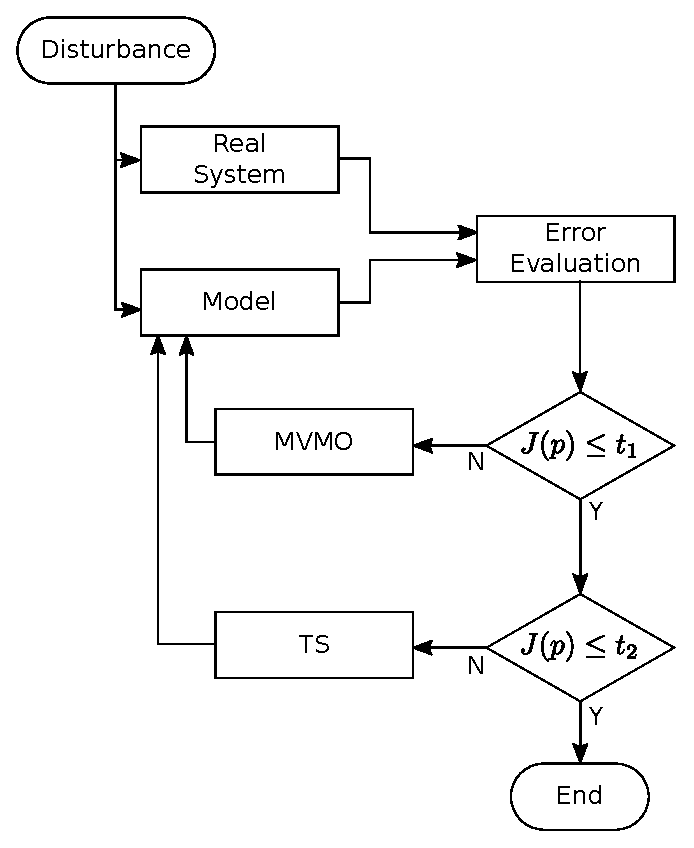
\includegraphics[scale=0.7]{Images/Flowchart.eps}
	\end{center}
	\label{fig: flowchart}
\end{figure}